\documentclass[accentcolor=tud7b,colorbacktitle,inverttitle,landscape,presentation,t]{tudbeamer}
\usepackage{graphicx} 
\usepackage{ngerman}
\usepackage[utf8]{inputenc}
\usepackage{booktabs}
\usepackage{wrapfig}
%\usepackage{caption}
%\usepackage{subcaption}
\usepackage{listings}
\renewcommand{\arraystretch}{1.2}
\usepackage{url}
\usepackage{tikz}
\usepackage{subfig}
\usepackage{pgfplots}
\pgfplotsset{compat=1.12} %width=7cm,
\usepackage{pgfplotstable}
%\usepackage{multimedia}
%\usepackage{movie9}
\usepackage{multirow}
\usepackage{rotating}


%\hypersetup{ colorlinks, citecolor=green, filecolor=black, linkcolor=blue, urlcolor=blue } 

\setbeamertemplate{section in toc}[square]
\setbeamertemplate{subsection in toc}[square]
\setbeamertemplate{bibliography item}{\insertbiblabel}
% \setbeamercolor{example text}{fg=green!50!black}
% \setbeamercolor{block alerted  item}{fg=red}

\setbeamercolor{block title alerted}{fg=red}
%body
%\setbeamercolor{block body alerted}{fg=black!90,bg=brown!60!yellow}
% parent of all alerts default is red
\setbeamercolor{alerted text}{fg=red}

\begin{document}

\title{Numerical Simulation of Compressible Flows with Immersed Boundaries Using Discontinuous Galerkin Methods}
\subtitle{Bachelor thesis by Simone Stange\\Prof. Dr.-Ing. habil. Martin Oberlack\\Betreuer: Dr.-Ing Björn Müller}

\author[Simone Stange]{Simone Stange}
\institute[fdy TUD]{Institut für Strömungsdynamik, TU Darmstadt}

\logo{
\includegraphics{img/fdy}}
% \logo{\color{tudtextaccent}\large IFP}

\date{\today}

\begin{titleframe}
	\begin{figure}[htbp] 
	    \centering
		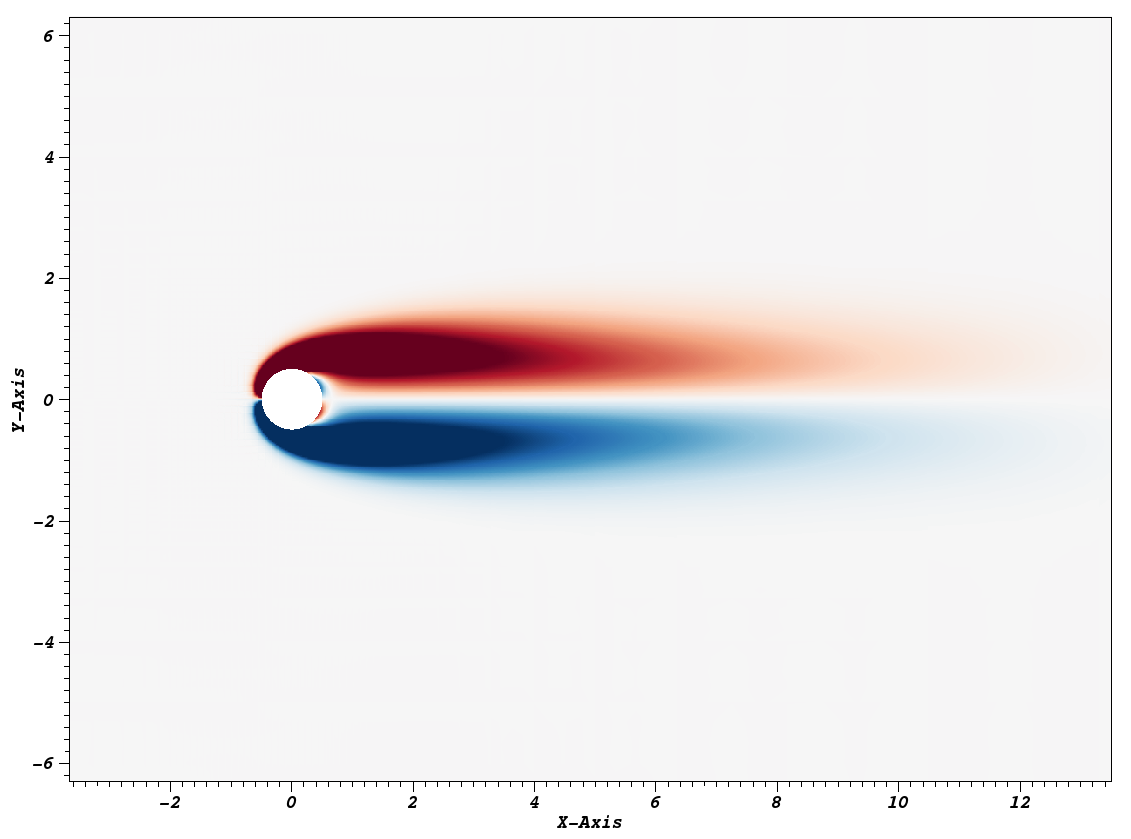
\includegraphics[height=0.38\textwidth]{img/Re40DG3CpD60} 
	\end{figure}
\end{titleframe}

\section*{Outline}
\begin{frame}
	\frametitle{Outline}
	\tableofcontents
\end{frame}
\section{Introduction and Fundamentals}
\frame{\tableofcontents[currentsection]}
	\subsection{Introduction}
	\begin{frame}
		\frametitle{Introduction}
		\begin{itemize}
			\item Aim of this thesis:
		\begin{itemize}
			\item Verification of CNS extension for BoSSS for inviscid flows
			\item Validation for viscid flows
			\item Both using immersed boundaries
		\end{itemize}
		\item CNS extension of BoSSS (Bounded Support Spectral Solver) numerically solves the Compressible Navier-Stokes equations using a Discontinuous Galerkin method
		\item CNS has already been verified and validated for:
		\begin{itemize}
			\item Inviscid flows using immersed boundaries by \cite[Müller 2014]{muller2014}, though not for the flow around a cylinder
			\item Viscid flows using curved elements by \cite[Ayers 2015]{ayers2015}
		\end{itemize}
		\end{itemize}
	\end{frame}
	\begin{frame}
		\frametitle{Flow Properties}
		\begin{itemize}
			\item Compressible flow
			\item Ideal gas 
			\begin{itemize}
				\item Heat capacity ratio $\gamma = \dfrac{c_p}{c_v} = 1.4$
			\end{itemize}
			\item Newtonian fluid
			\begin{itemize}
				\item Stress tensor $\tau_{ij} = \mu \left[\left(\dfrac{\partial u_i}{\partial x_j} + \dfrac{\partial u_j}{\partial x_i}\right)- \dfrac{2}{3}\dfrac{\partial u_k}{\partial x_k} \delta_{ij}\right]$
			\end{itemize}
			\item Mach number $\text{Ma} = \dfrac{v_\infty}{a_\infty} = 0.2$
			\item Reynolds number $\text{Re} = \dfrac{\rho_\infty V_\infty L}{\mu_\infty} \propto \dfrac{\text{inertia forces}}{\text{viscous forces}}$
			\item Prandtl number $\text{Pr} = \dfrac{ \mu_\infty c_p}{k_\infty} \propto \dfrac{\text{viscous diffusion rate}}{\text{thermal diffusion rate}}$
		\end{itemize}
	\end{frame}
	\begin{frame}
		\frametitle{Non-dimensional 2D Compressible Navier-Stokes Equations}

%		time discretisation durch Runge-Kutta erster Ordnung -> expliziter Euler
\vspace{-0.5cm}
\begin{itemize}
	\item 2D
	\item Non-dimensional conserved flow variables: density $\rho$, momentum $\rho u$, $\rho v$, energy $\rho E$
\end{itemize}
\vspace{-0.3cm}
	\scalebox{0.9}{
		\begin{minipage}{\the\textwidth}
		\begin{align*}
			\tcbhighmath[drop fuzzy shadow,colframe=myblue]{\dfrac{\partial U}{\partial t}}+\tcbhighmath[drop fuzzy shadow,colframe=mygreen]{ \left(\dfrac{\partial F_c^x(U)}{\partial x} + \dfrac{\partial F_c^y(U)}{\partial y}\right)} - \tcbhighmath[drop fuzzy shadow,colframe=myred]{\left( \dfrac{\partial F_v^x(U, \nabla U)}{\partial x} + \dfrac{\partial F_v^y(U, \nabla U}{\partial y}\right)} = 0 			
		\end{align*}
	\end{minipage}
	}
	\begin{columns}[t]
		\begin{column}{0.6\textwidth}
			%\column[t]{7cm}
			\scalebox{0.75}{
			\begin{minipage}{\the\textwidth}
			\begin{flalign*}
			U &=\left(\begin{array}{c} \rho\\	\rho u\\ \rho v\\ \rho E\\	\end{array} \right) \quad 
			F_c^x=\left(\begin{array}{c} \rho u\\	\rho u^2 +p\\ \rho u v\\ u(\rho E +p)\\	\end{array} \right) \quad 
			F_c^y=\left(\begin{array}{c} \rho v\\	\rho u v\\ \rho v^2 +p\\ v(\rho E +p)\\	\end{array} \right) \\[8pt]
			F_v^x &= \dfrac{1}{\text{Re}}\left(\begin{array}{c} 0\\	\tau_{xx}\\ \tau_{xy}\\ \tau_{xx} u + \tau_{xy} v + \dfrac{\gamma}{\text{Pr}(\gamma - 1)}\kappa\dfrac{\partial T}{\partial x}\\	\end{array} \right) \quad
			F_v^y = \dfrac{1}{\text{Re}}\left(\begin{array}{c} 0\\	\tau_{xy}\\ \tau_{yy}\\ \tau_{xy} u + \tau_{yy} v + \dfrac{\gamma}{\text{Pr}(\gamma - 1)}\kappa\dfrac{\partial T}{\partial y}\\	\end{array} \right)
			\end{flalign*}			
		\end{minipage}
	}
	\end{column}
	\begin{column}{0.35\textwidth}
		%	\column[t]{5cm}
	\vspace{-2cm}
	\begin{itemize}
		\bluedot Temporal derivative
		\greendot Convective fluxes
		\reddot Viscous fluxes
	\end{itemize}
\end{column}
\end{columns}

	\end{frame}
	\subsection{The Discontinuous Galerkin Method}
	\begin{frame}
		\frametitle{The Discontinuous Galerkin Space Discretisation}
		\begin{columns}[t]
			\column[]{8.2cm}
			\vspace{-0.5cm}
			\begin{itemize}
				\item Discrete weak formulation of $\dfrac{\partial c}{\partial t} + \nabla \cdot \boldsymbol{f}(c) = 0 $
				\item Discretisation $\Omega_h$ of $\Omega$
				\item Multiplication of PDE by set of cell-local test functions $\Phi_{i,j}$
				\item Integration over cell $\mathcal{K}_i$ and integration by parts
				\item Modal approximation for $c(\mathbf{x} , t)\mid _{\mathcal{K}_i} \approx \sum_{k = 0}^{M}c_{i,k}(t) \Phi_{i,k}(\mathbf{x})$ with Galerkin approach (identical Ansatz and test functions)
				\item Discontinuous approach \MVRightArrow \, flux function $f = f(c^-, c^+, \mathbf{n})$
			\end{itemize}
			\vspace{-0.3cm}
			\scalebox{0.8}{
			\begin{minipage}{\the\textwidth}
			\begin{align*}
			\Rightarrow \int\limits_{\mathcal{K}_i} \dfrac{\partial c_i}{\partial t}\Phi_{i,j} \, dV +
			\sum_{e=1}^{E_i}\int\limits_{\mathcal{E}_{i,e}} f \left( c^-, c^+, \mathbf{n} \right) \Phi_{i,j} \, dA - \int\limits_{\mathcal{K}_i} \boldsymbol{f}\left(c_i\right) \cdot \nabla\Phi_{i,j} \, dV = 0
			\end{align*}
		\end{minipage}
	}
			\column[]{3.8cm}
			\begin{figure}[ht]
				%\centering
				\vspace{-1cm}
				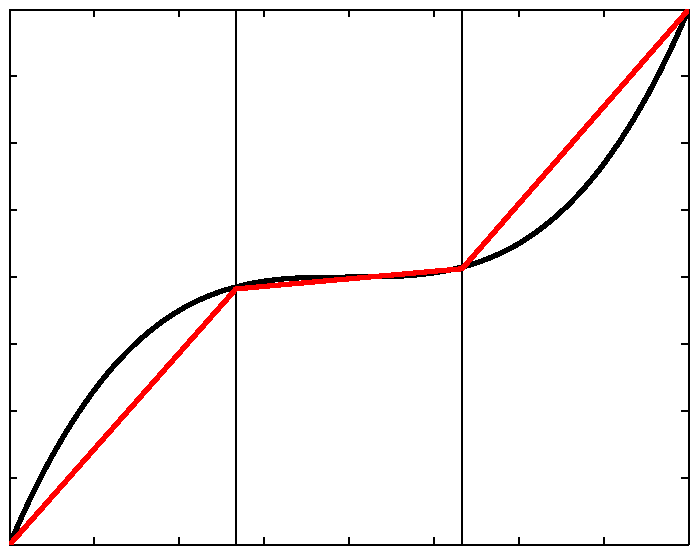
\includegraphics[height=0.31\textheight]{img/fem_cropped.pdf}
			%	\caption{First order FEM}
			\end{figure}
			\begin{figure}[htbp]
				\vspace{-0.6cm}
				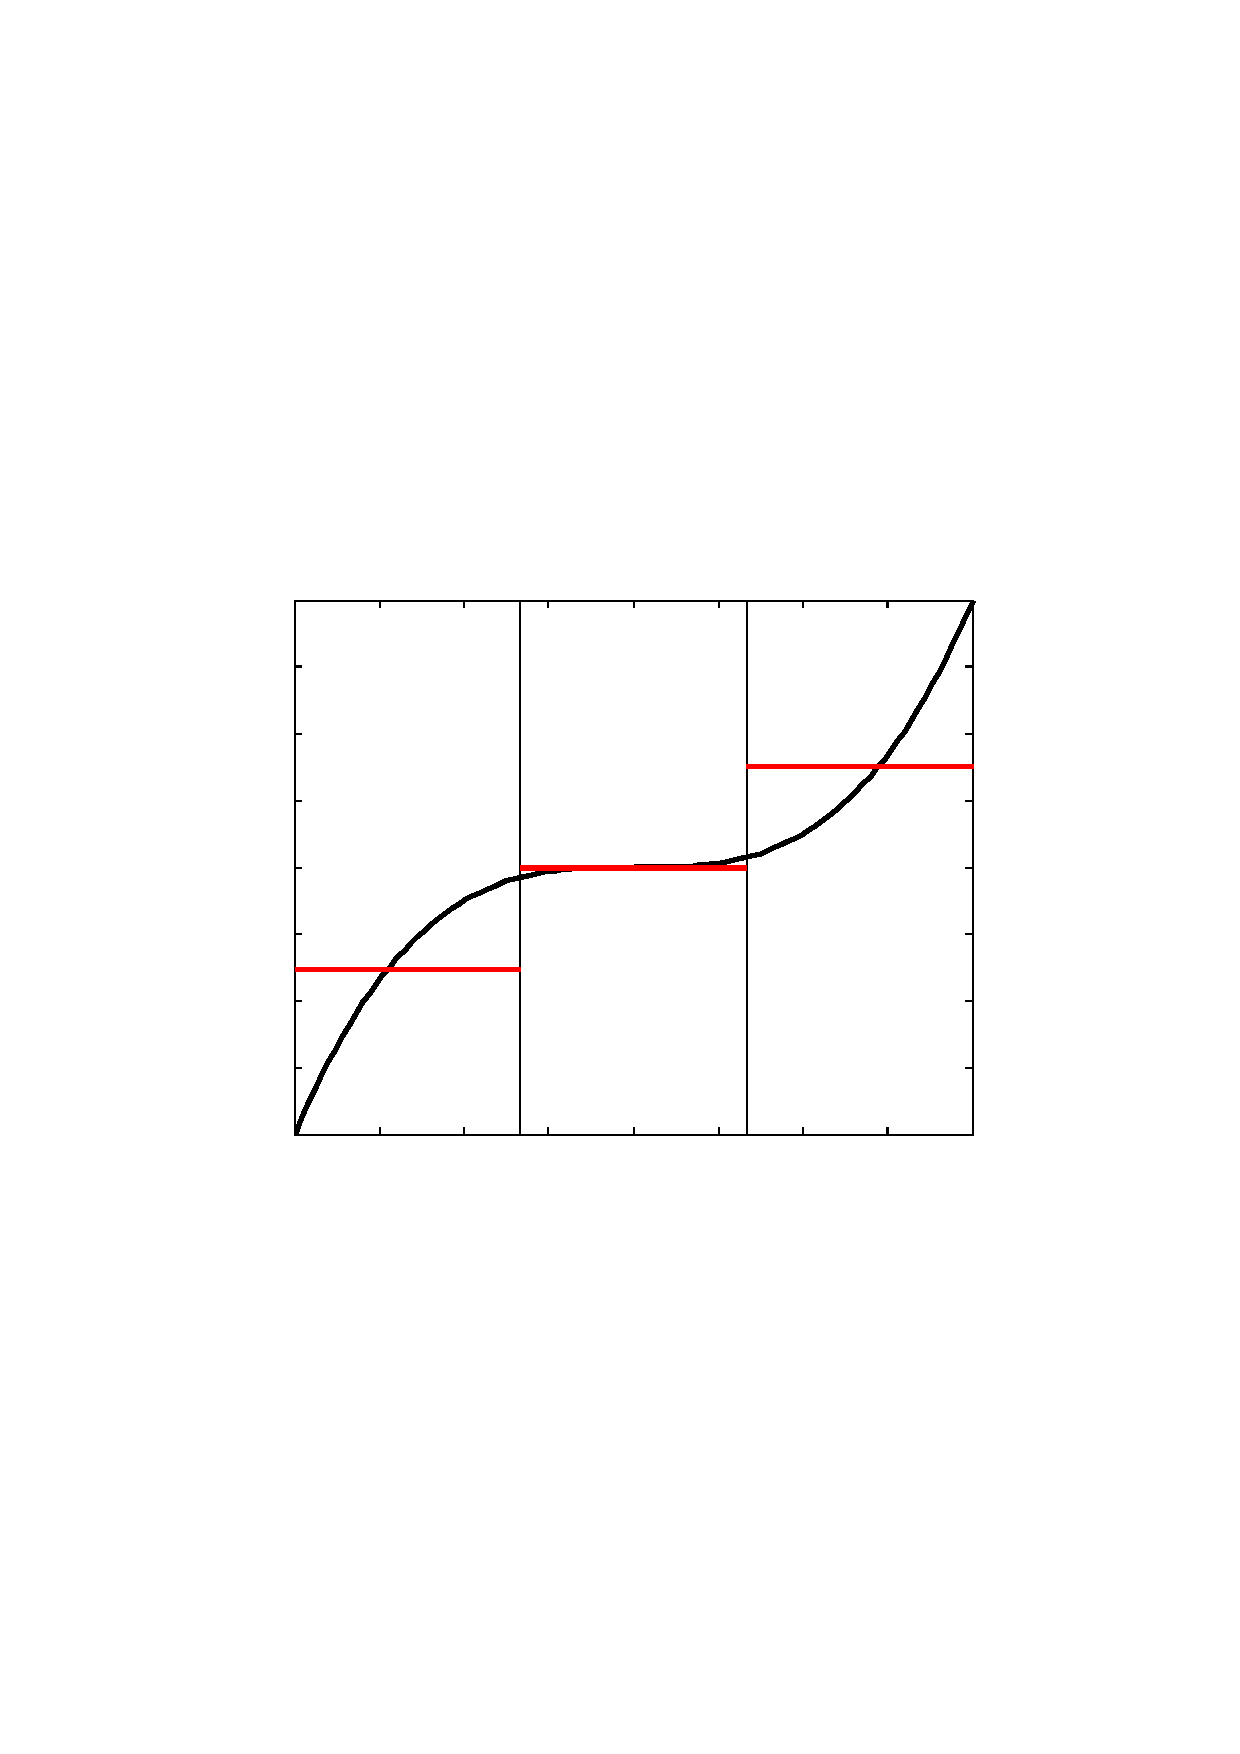
\includegraphics[height=0.31\textheight]{img/fvm.pdf}
				%\caption{Zeroth order DG (FVM) }
			\end{figure} 
			\begin{figure}[htbp]
				\vspace{-0.6cm}
				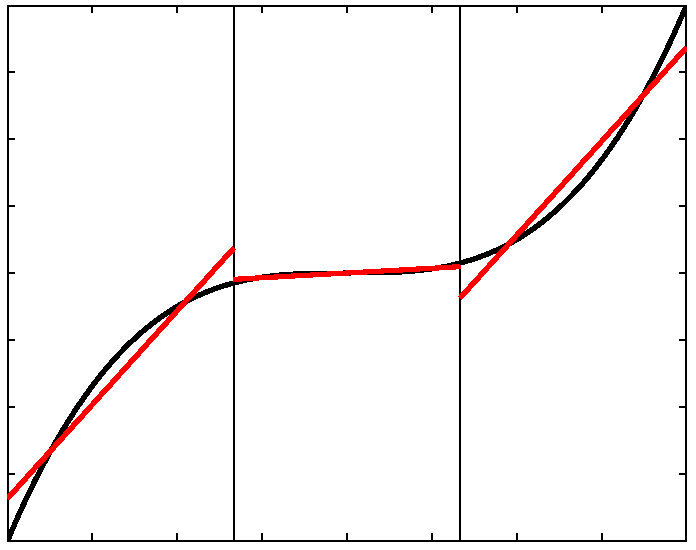
\includegraphics[height=0.31\textheight]{img/dg.pdf}
				\vspace{-0.1cm}
				\caption{Adapted from \cite{muller2014}}
			\end{figure} 
		\end{columns}
	\end{frame}
%		\begin{figure}
%			\centering
%			\subfloat[First order FEM \label{fig:a}]{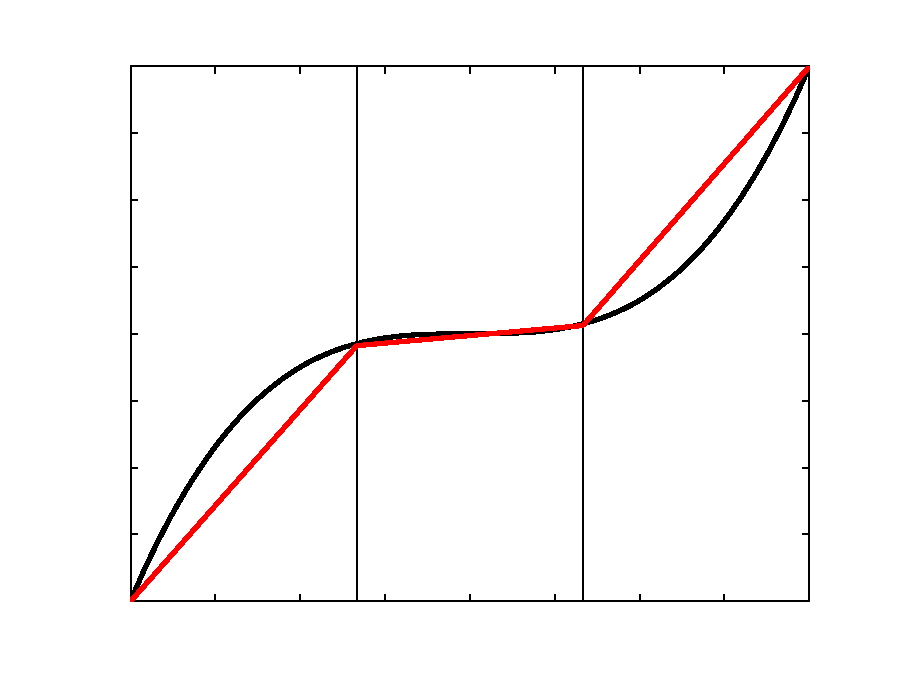
\includegraphics[width=0.28\textwidth]{img/fem.eps}}
%			\subfloat[Zeroth order DG (FVM)\label{fig:b}]{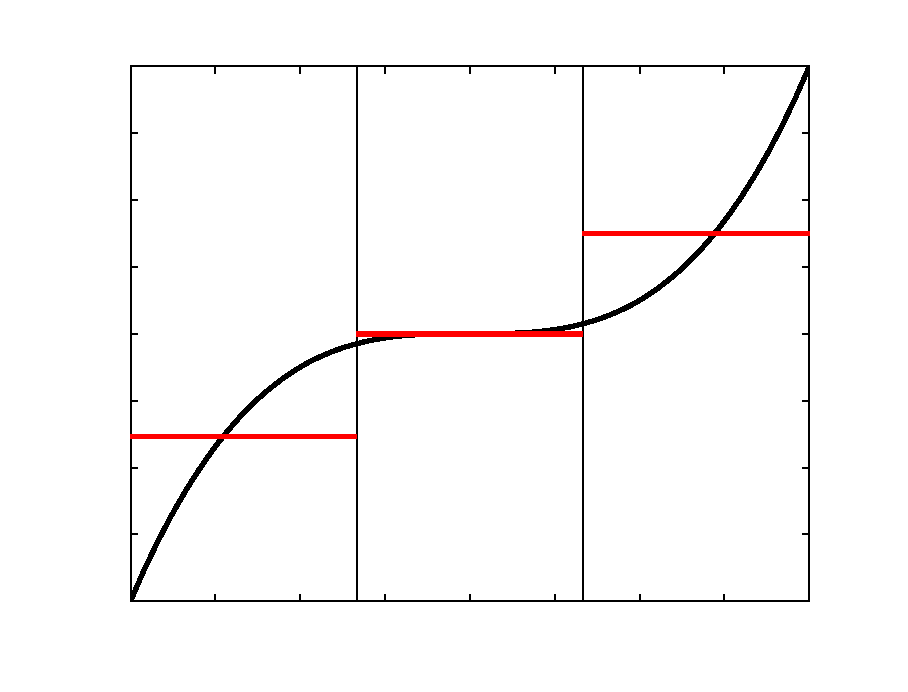
\includegraphics[width=0.28\textwidth]{img/fvm.eps}}
%			\subfloat[First order DG \label{fig:c}]{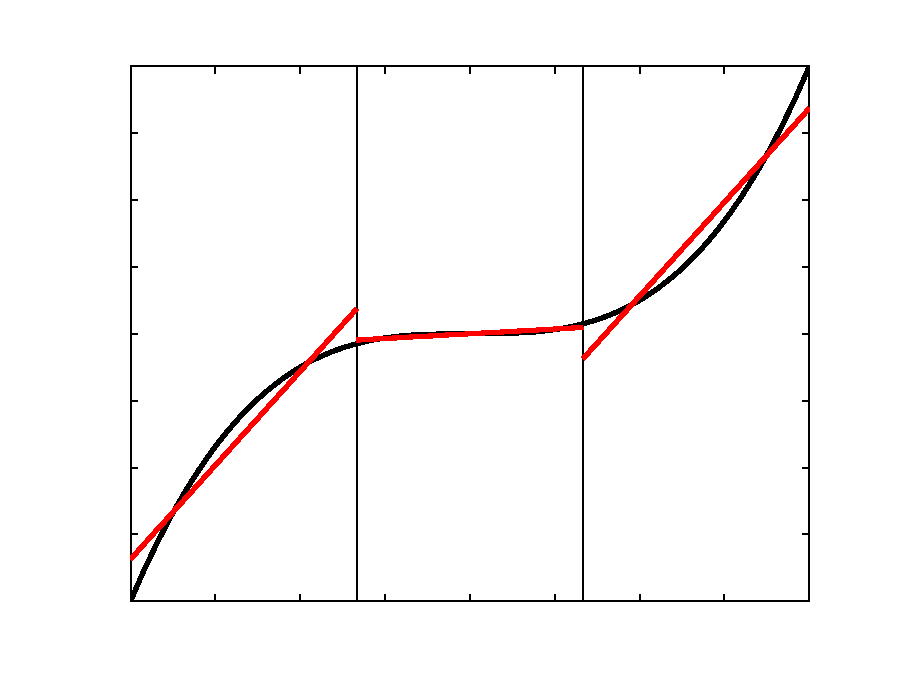
\includegraphics[width=0.28\textwidth]{img/dg.eps}}
%			\caption{Comparison of FEM, FVM and DG}
%			\label{fig:1}
%		\end{figure}
%		\begin{itemize}
%			\item Discrete weak formulation of $\dfrac{\partial c}{\partial t} + \nabla \cdot \boldsymbol{f}(c) &= 0 $
%			\item Discretisation $\Omega_h$ of $\Omega$
%			\item Multiplication of PDE by set of cell-local test functions
%			\item Integration over cell $\mathcal{K}_i$ and integration by parts
%			\item Modal approximation for $c(\mathbf{x} , t)\mid _{\mathcal{K}_i} \approx \sum_{k = 0}^{M}c_{i,k}(t) \Phi_{i,k}(\mathbf{x})$ with Galerkin approach (identical Ansatz and test functions)
%			\item Discontinuous approach \MVRightArrow \, flux function $f = f(c^-, c^+, \mathbf{n})$
%		\end{itemize}

%		DG space discretisation Vorgehen, Bildchen, fluxes

	\subsection{The Immersed Boundary Method}
	\begin{frame}
		\frametitle{The Immersed Boundary Method}
		\begin{columns}[t]
			\column[]{7cm}
			\vspace{-0.5cm}
			\begin{itemize}
				\item Division into
					\begin{itemize}
						\item the physical region:  $\mathcal{A} = \left\{\vec{x} \in \Omega_h : \varphi (\vec{x}) > 0 \right\}$,
						\item the void region:  $\mathcal{B} = \left\{ \vec{x}\in \Omega_h : \varphi (\vec{x}) < 0 \right\}$, 
						\item the immersed boundary: $\mathcal{I} = \left\{ \vec{x}\in \Omega_h : \varphi (\vec{x}) = 0 \right\}$
					\end{itemize} 
			\end{itemize}
			\column[]{5cm}
			\begin{figure}[htbp]
				\vspace{-1cm}
				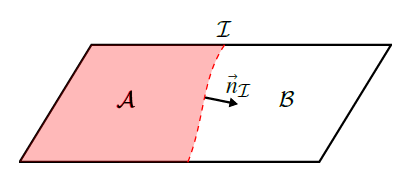
\includegraphics[width=\textwidth]{img/ibmcut.PNG}
				\caption{Cut cell with physical (red) and void region (white) \cite{paper}}\label{fig:cutcell}
			\end{figure} 
		\end{columns}
		\begin{itemize}
			\item Restrict problem domain to physical region:
		\end{itemize}
		\vspace{-0.3cm}
		\scalebox{0.9}{
			\begin{minipage}{\the\textwidth}			
				\begin{align*}
				\int\limits_{\mathcal{A}_i} \dfrac{\partial c_i}{\partial t}\Phi_{i,j} \, dV +
				\sum_{e=1}^{E_i}\int\limits_{\mathcal{E}_{i,e}^\mathcal{A}} f \left( c^-, c^+, \mathbf{n} \right) \Phi_{i,j} \, dA + \int\limits_{\mathcal{I}_{i}} f \left( c^-, c^+, \mathbf{n}_\mathcal{I} \right) \Phi_{i,j} \, dA - \int\limits_{\mathcal{A}_i} \boldsymbol{f}\left(c_i\right) \cdot \nabla\Phi_{i,j} \, dV = 0 
				\end{align*}
			\end{minipage}
			}\\
			\begin{itemize}
				\item Solution via explicit Euler time discretisation
					\begin{itemize}
						\item Time step size depends on cell with smallest volume \\
						\MVRightarrow \, Cell agglomeration
					\end{itemize}
			\end{itemize}
%		regions mit Bild, Aufteilung Integrale
%		mass matrix
%		rk time discretisation formel
%		cell agglomeration
	\end{frame}
	\begin{frame}
		\frametitle{Cell Agglomeration}

		\begin{columns}[t]
			\column[]{5cm}
			\vspace{-0.5cm}
			\begin{itemize}
				\item Agglomeration threshold  $0 \leq \alpha \leq 1$
				\item Cells $\mathcal{K}_s^\text{src}$ with $\text{frac}(\mathcal{A}_i) = \tfrac{\text{meas}(\mathcal{A}_i)}{\text{meas}(\mathcal{K}_i)} \leq \alpha$ get agglomerated to neighbouring cell $\mathcal{K}_s^\text{tar}$
				\item Neighbouring cells are weakly coupled via fluxes \newline \MVRightArrow \, basis $\vec{\Phi}_i$ can be extended from the target cell into the source cell
			\end{itemize}
			\column[]{7cm}
			\begin{figure}[htbp]
				\vspace{-1cm}
				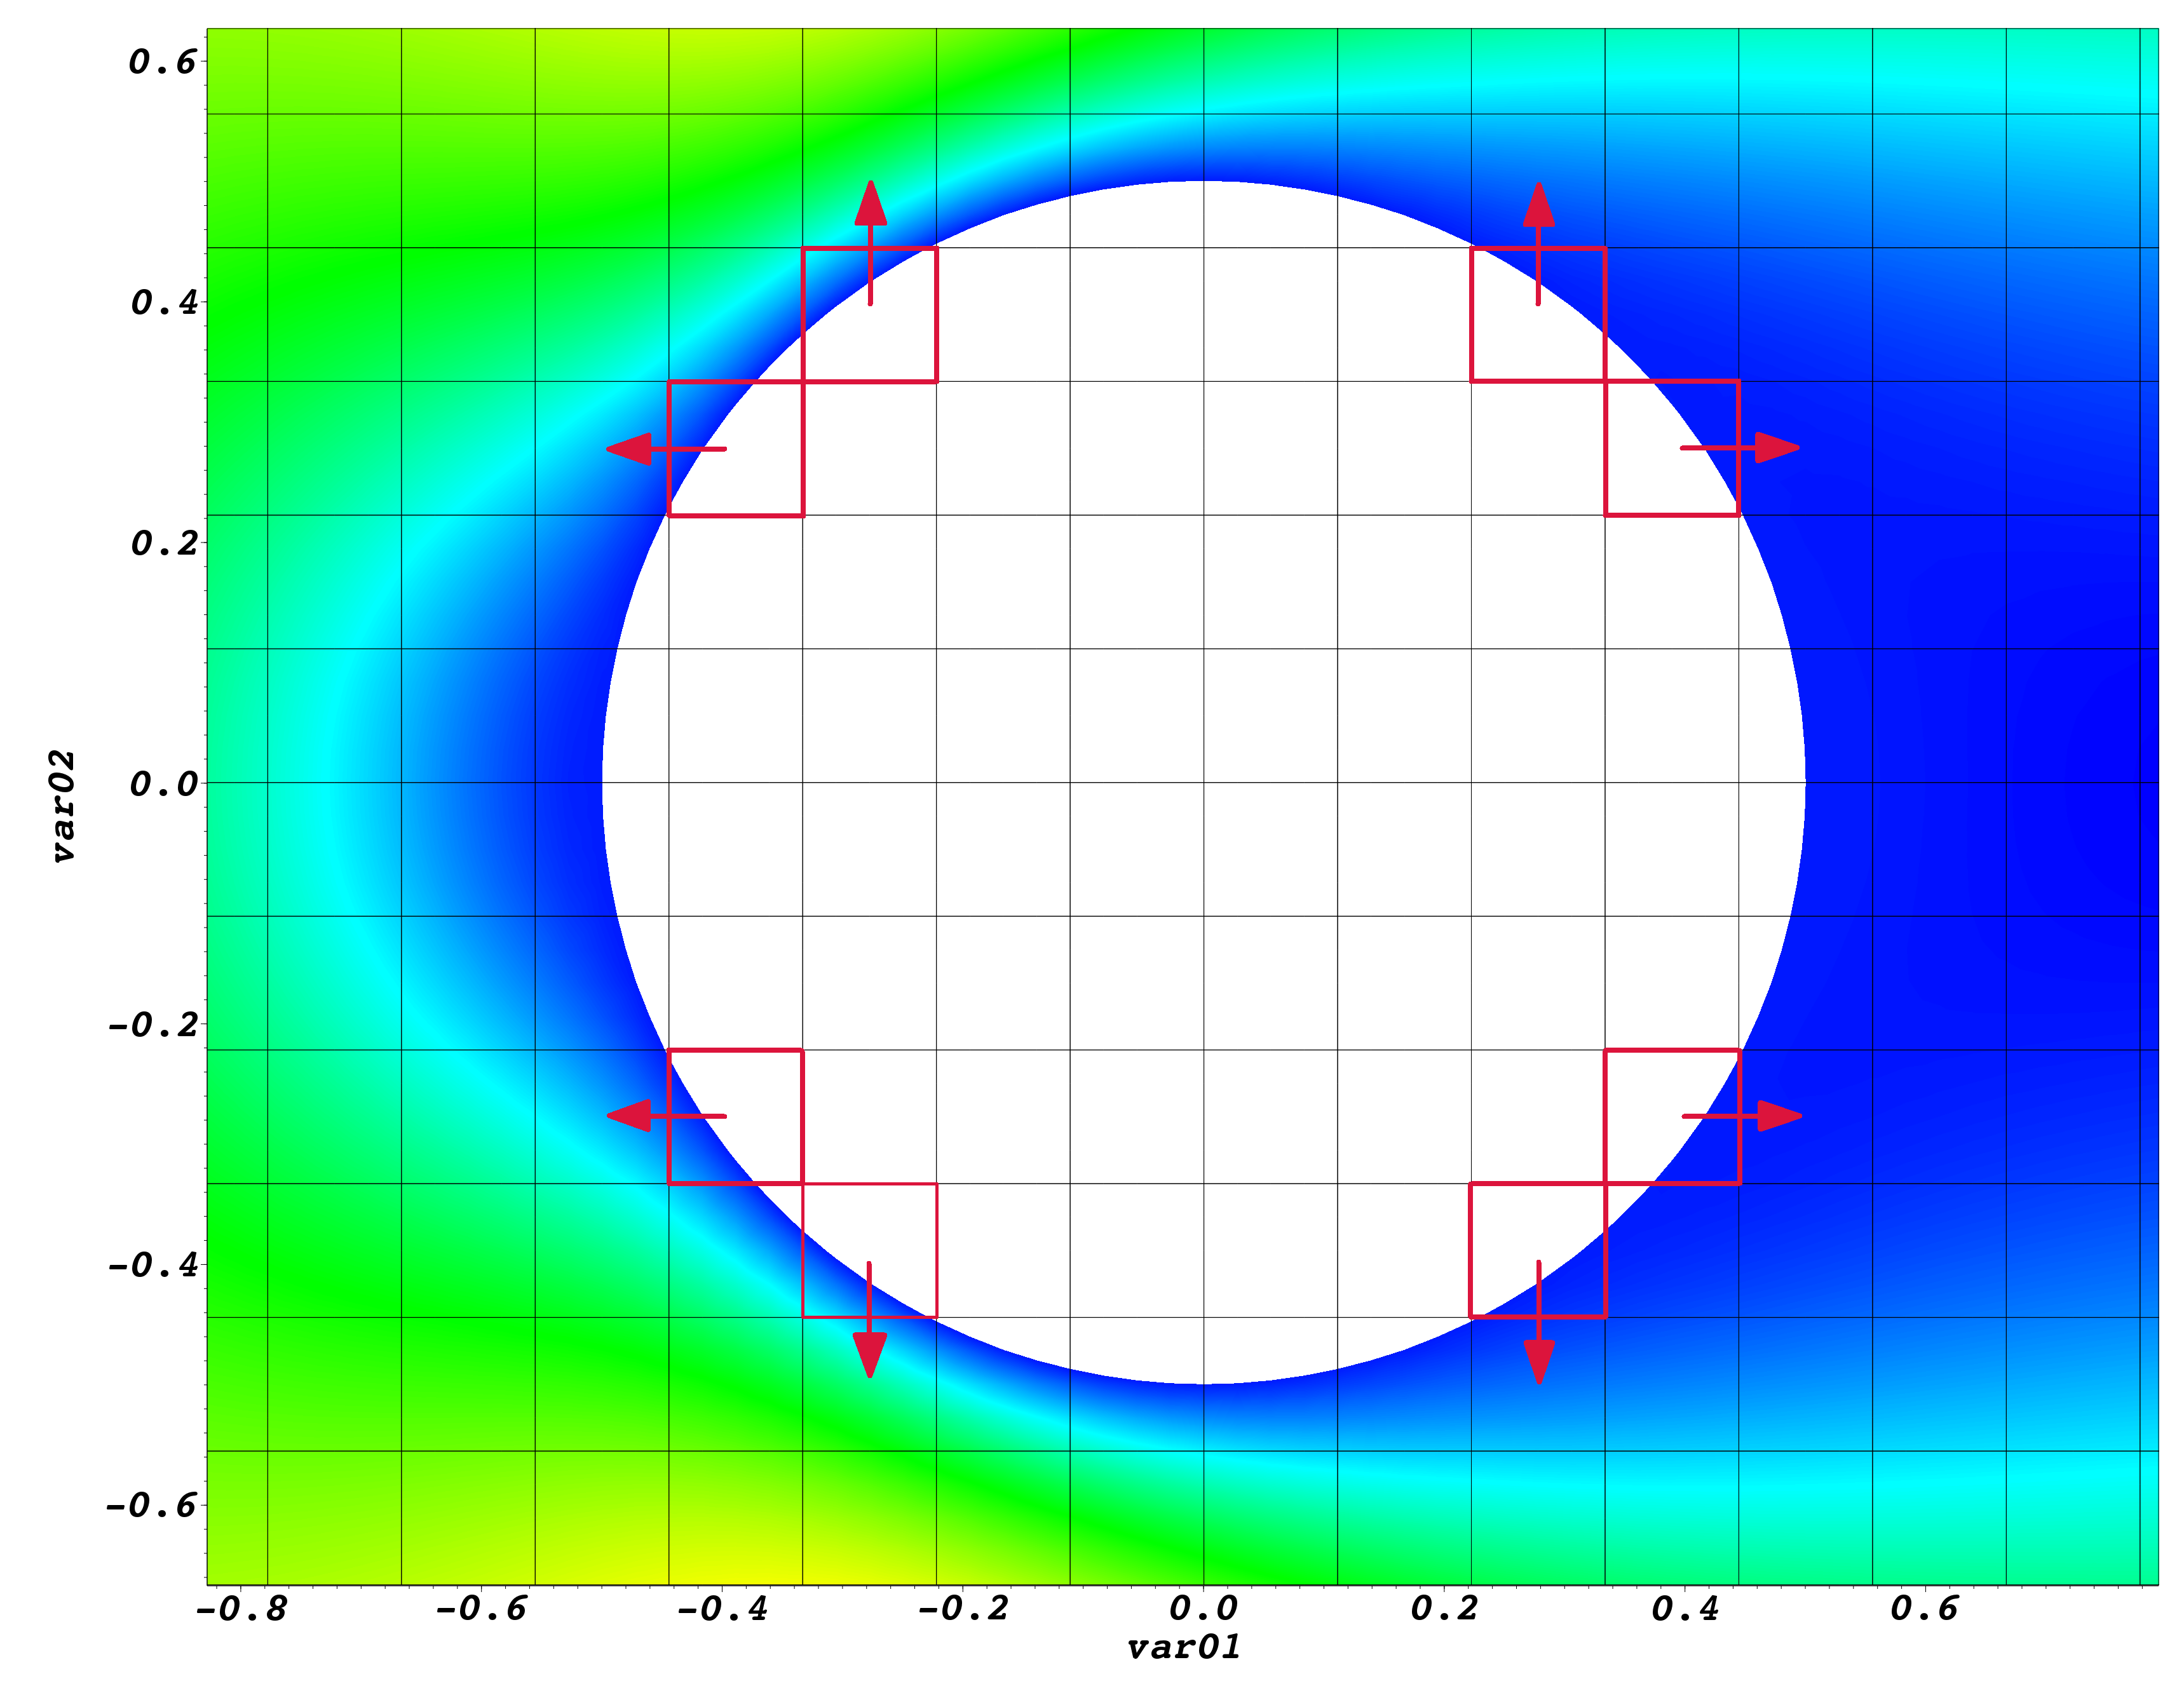
\includegraphics[width=\textwidth]{img/agglom.PNG}
				\caption{Cell agglomeration for $\alpha = 0.3$}
			\end{figure} 
		\end{columns}
%		regions mit Bild, Aufteilung Integrale
%		mass matrix
%		rk time discretisation formel
%		cell agglomeration
	\end{frame}
\section{Verification of BoSSS for Inviscid Flows}
\frame{\tableofcontents[currentsection]}
\begin{frame}
	\frametitle{Problem Specification}
Gitter, Bild, domain, level set, isentropic inviscid flow mit gleichung -> s=0
\end{frame}
	\subsection{Robustness}
	\begin{frame}
		\frametitle{Robustness Study -- Preparation}
		shift, degree 1 bis 3, agglo 0.5, 64 mal 64 cells
		Parameter, was wird getan
	\end{frame}
	\begin{frame}
		\frametitle{Robustness Study -- Evaluation}
			\begin{figure}[htp]	
				\centering
				\begin{tikzpicture}
				\begin{semilogyaxis}[xlabel ={Position of Centre Point of the Cylinder}, ylabel ={$L_2$ Error of Entropy}, grid =major, legend entries ={$P=1$,$P=2$, $P=3$}, unbounded coords=jump, legend style = {cells = {anchor=east}, legend pos=outer north east,}, scaled x ticks = false]
				\addplot table[ x =shift, y =error1] {data/shift.dat};
				\addplot table[ x =shift, y =error2] {data/shift.dat};
				\addplot table[ x =shift, y =error3] {data/shift.dat};
				\end{semilogyaxis}	
				\end{tikzpicture}
				\caption{Convergence Plot}
				\label{shifterror}
			\end{figure}
		Ergebnisse, Plot, komischer punkt wird angeschaut
	\end{frame}
	\subsection{Convergence}
	\begin{frame}
		\frametitle{Comvergence Study -- Preparation}
		Parameter, was wird getan
	\end{frame}
	\begin{frame}
		\frametitle{Convergence Study -- Evaluation}
		\begin{figure}[htp]
			\centering		
			\begin{tikzpicture}
			\begin{loglogaxis}[xlabel ={Cells per Direction}, ylabel ={$L_2$ Error of Entropy}, grid =major, legend entries ={$P=0$,$P=1$,$P=2$, $P=3$, $P=4$, $R_0$, $R_1$, $R_2$, $R_3$, $R_4$}, unbounded coords=jump, legend style = {cells = {anchor=east}, legend pos=outer north east}]
			\addplot table[ x =meshSize, y =error0] {data/test.dat};
			\addplot table[ x =meshSize, y =error1] {data/test.dat};
			\addplot table[ x =meshSize, y =error2] {data/test.dat};
			\addplot table[ x =meshSize, y =error3] {data/test.dat};
			\addplot table[ x =meshSize, y =error4] {data/test.dat};
			\addplot table[
			x=meshSize,
			y={create col/linear regression={						y=error0,}}	]
			{data/test.dat}
			coordinate[pos=0.6] (A)
			coordinate[pos=0.75] (B);
			\xdef\nullslope{\pgfplotstableregressiona}
			\draw (A) -| (B)
			node [pos=0.75, anchor = south west] {\pgfmathprintnumber[fixed]{\nullslope}};
			\addplot table[
			x=meshSize,
			y={create col/linear regression={						y=error1,}}	]
			{data/test.dat}
			coordinate[pos=0.6] (A)
			coordinate[pos=0.75] (B);
			\xdef\einsslope{\pgfplotstableregressiona}
			\draw (A) -| (B)
			node [pos=0.75, anchor = west] {\pgfmathprintnumber{\einsslope}};
			\addplot table[
			x=meshSize,
			y={create col/linear regression={						y=error2,}}	]
			{data/test.dat}
			coordinate[pos=0.6] (A)
			coordinate[pos=0.75] (B);
			\xdef\zweislope{\pgfplotstableregressiona}
			\draw (A) -| (B)
			node [pos=0.75, anchor = west] {\pgfmathprintnumber{\zweislope}};
			\addplot table[
			x=meshSize,
			y={create col/linear regression={						y=error3,}}	]
			{data/test.dat}
			coordinate[pos=0.6] (A)
			coordinate[pos=0.75] (B);
			\xdef\dreislope{\pgfplotstableregressiona}
			\draw (A) -| (B)
			node [pos=0.75, anchor = west] {\pgfmathprintnumber{\dreislope}};
			\addplot table[
			x=meshSize,
			y={create col/linear regression={						y=error4,}}	]
			{data/test.dat}
			coordinate[pos=0.6] (A)
			coordinate[pos=0.75] (B);
			\xdef\vierslope{\pgfplotstableregressiona}
			\draw (A) -| (B)
			node [pos=0.75, anchor = west] {\pgfmathprintnumber{\vierslope}};
			\end{loglogaxis}	
			\end{tikzpicture}	
			\caption{Convergence Plot}
			\label{mesherror}
		\end{figure}
		Ergebnisse, Plot
	\end{frame}
\section{Evaluation of BoSSS for Viscid Flows}
\frame{\tableofcontents[currentsection]}
	\subsection{Theory}
	\begin{frame}
		\frametitle{Theory -- Viscid Flow Around a Cylinder}
		\begin{columns}[t]
			\column[]{6cm}
			\vspace{-0.5cm}
			\begin{itemize}
				\item $\text{Re} \leq 40-50$: laminar steady regime
				\item $40-50 \leq \text{Re} \leq 190$: laminar vortex shedding (Kármán vortex street)
				\item $190 \leq \text{Re}$: increasing 3D effects
				\pause
				\item Characteristic values:
				\begin{itemize}
					\item Coefficient of drag $C_D$
					\item Coefficient of lift $C_L$
					\item Wake separation length $W^*$
					\item Strouhal number (frequency of vortex shedding)
				\end{itemize}
			\end{itemize}
			\column[]{6cm}
			\onslide
			\begin{figure}[ht]
				%\centering
				 \vspace{-1cm}
				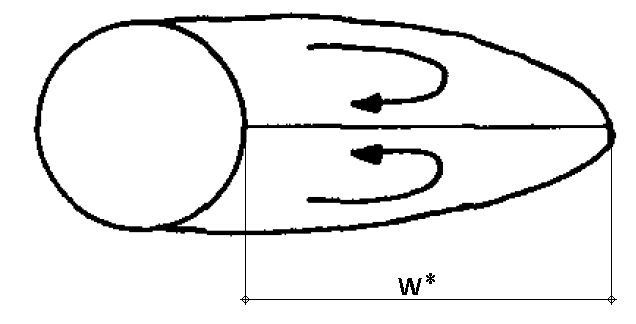
\includegraphics[width=0.6\textwidth]{img/steadyFlow_modifiedWilliamson.PNG}
				\caption{Laminar steady regime \cite{williamson} }
			\end{figure}
			\begin{figure}[htbp]
				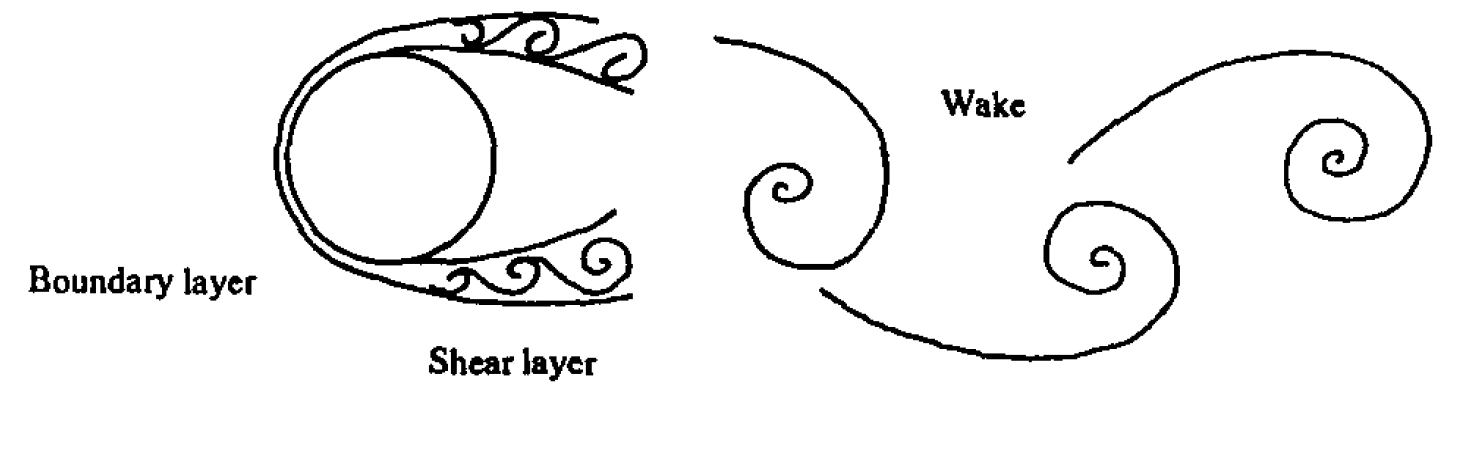
\includegraphics[width=\textwidth]{img/unsteady_Williamson.PNG}
				\caption{Kármán Vortex Street \cite{williamson} }
			\end{figure} 
		\end{columns}
	\end{frame}
%	\begin{frame}
%		\frametitle{Theory -- Laminar Steady Regime}
%		laminar steady regime
%		Bild
%		\begin{columns}[t]
%		\column[]{7cm}
%		\column[]{5cm}
%		\begin{figure}[htbp]
%			\vspace{-1cm}
%			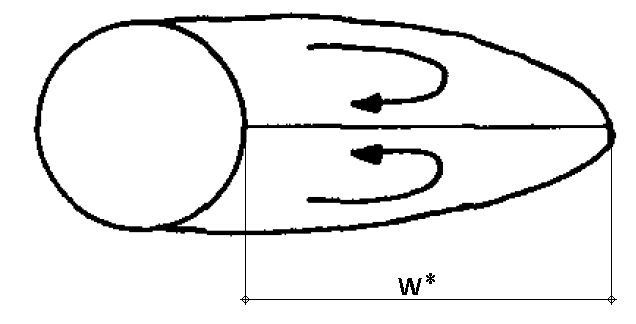
\includegraphics[width=\textwidth]{img/steadyFlow_modifiedWilliamson.PNG}
%			\caption{Recirculation Area \cite{williamson}}
%		
%		\end{figure} 
%		\end{columns}
%
%	\end{frame}	
%	\begin{frame}
%		\frametitle{Theory -- Laminar Vortex Shedding}
%		Bild
%		\begin{columns}[t]
%			\column[]{5cm}
%			\column[]{7cm}
%			\begin{figure}[htbp]
%				\vspace{-1cm}
%				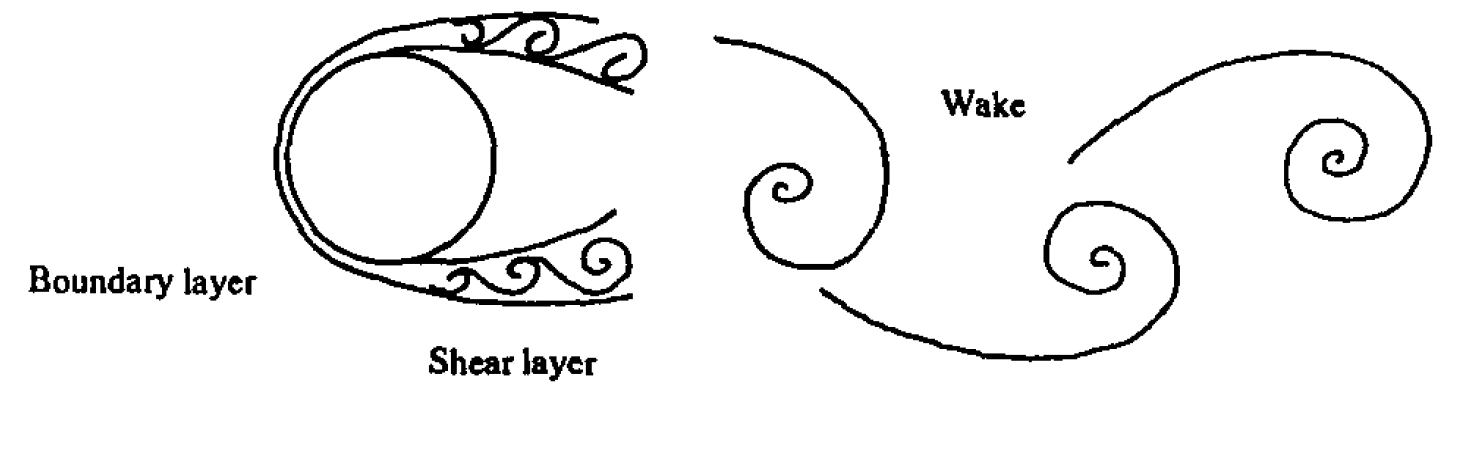
\includegraphics[width=\textwidth]{img/unsteady_Williamson.PNG}
%				\caption{Kármán Vortex Street \cite{williamson} }
%			\end{figure} 
%		\end{columns}
%		Karman vortex street
%		frequency /strouhal
%	\end{frame}	
	\subsection{Simulations}
		\begin{frame}
			\frametitle{Simulation Properties}
			\begin{columns}[t]
				\column[]{7cm}
				\vspace{-0.5cm}
			\begin{itemize}
				\item Domain:
				\begin{itemize}
					\item $-20 \leq x \leq 20$
					\item $-20 \leq y \leq 20$
					\item Cylinder with radius $r=0.5$ at $(0,0)$ \newline \MVRightarrow \, Level set $\varphi  = x^2 + y^2 -0.25$ set as  \color{myred} isothermal wall \color{black}
				\end{itemize}
				\pause
				\item Variation of mesh size: 40, 60 and 80 cells per direction
				\pause
				\item Variation of polynomial degree $1 \leq P \leq 3$
				\pause
				\item Constant agglomeration threshold $\alpha = 0.3$ \\[10pt]
				\onslide
				\bluedot Supersonic inlet
				\reddot Isothermal wall
			\end{itemize}
			\column[]{5.5cm}
			\onslide
			\vspace{-0.8cm}
			\begin{figure}[htbp]
				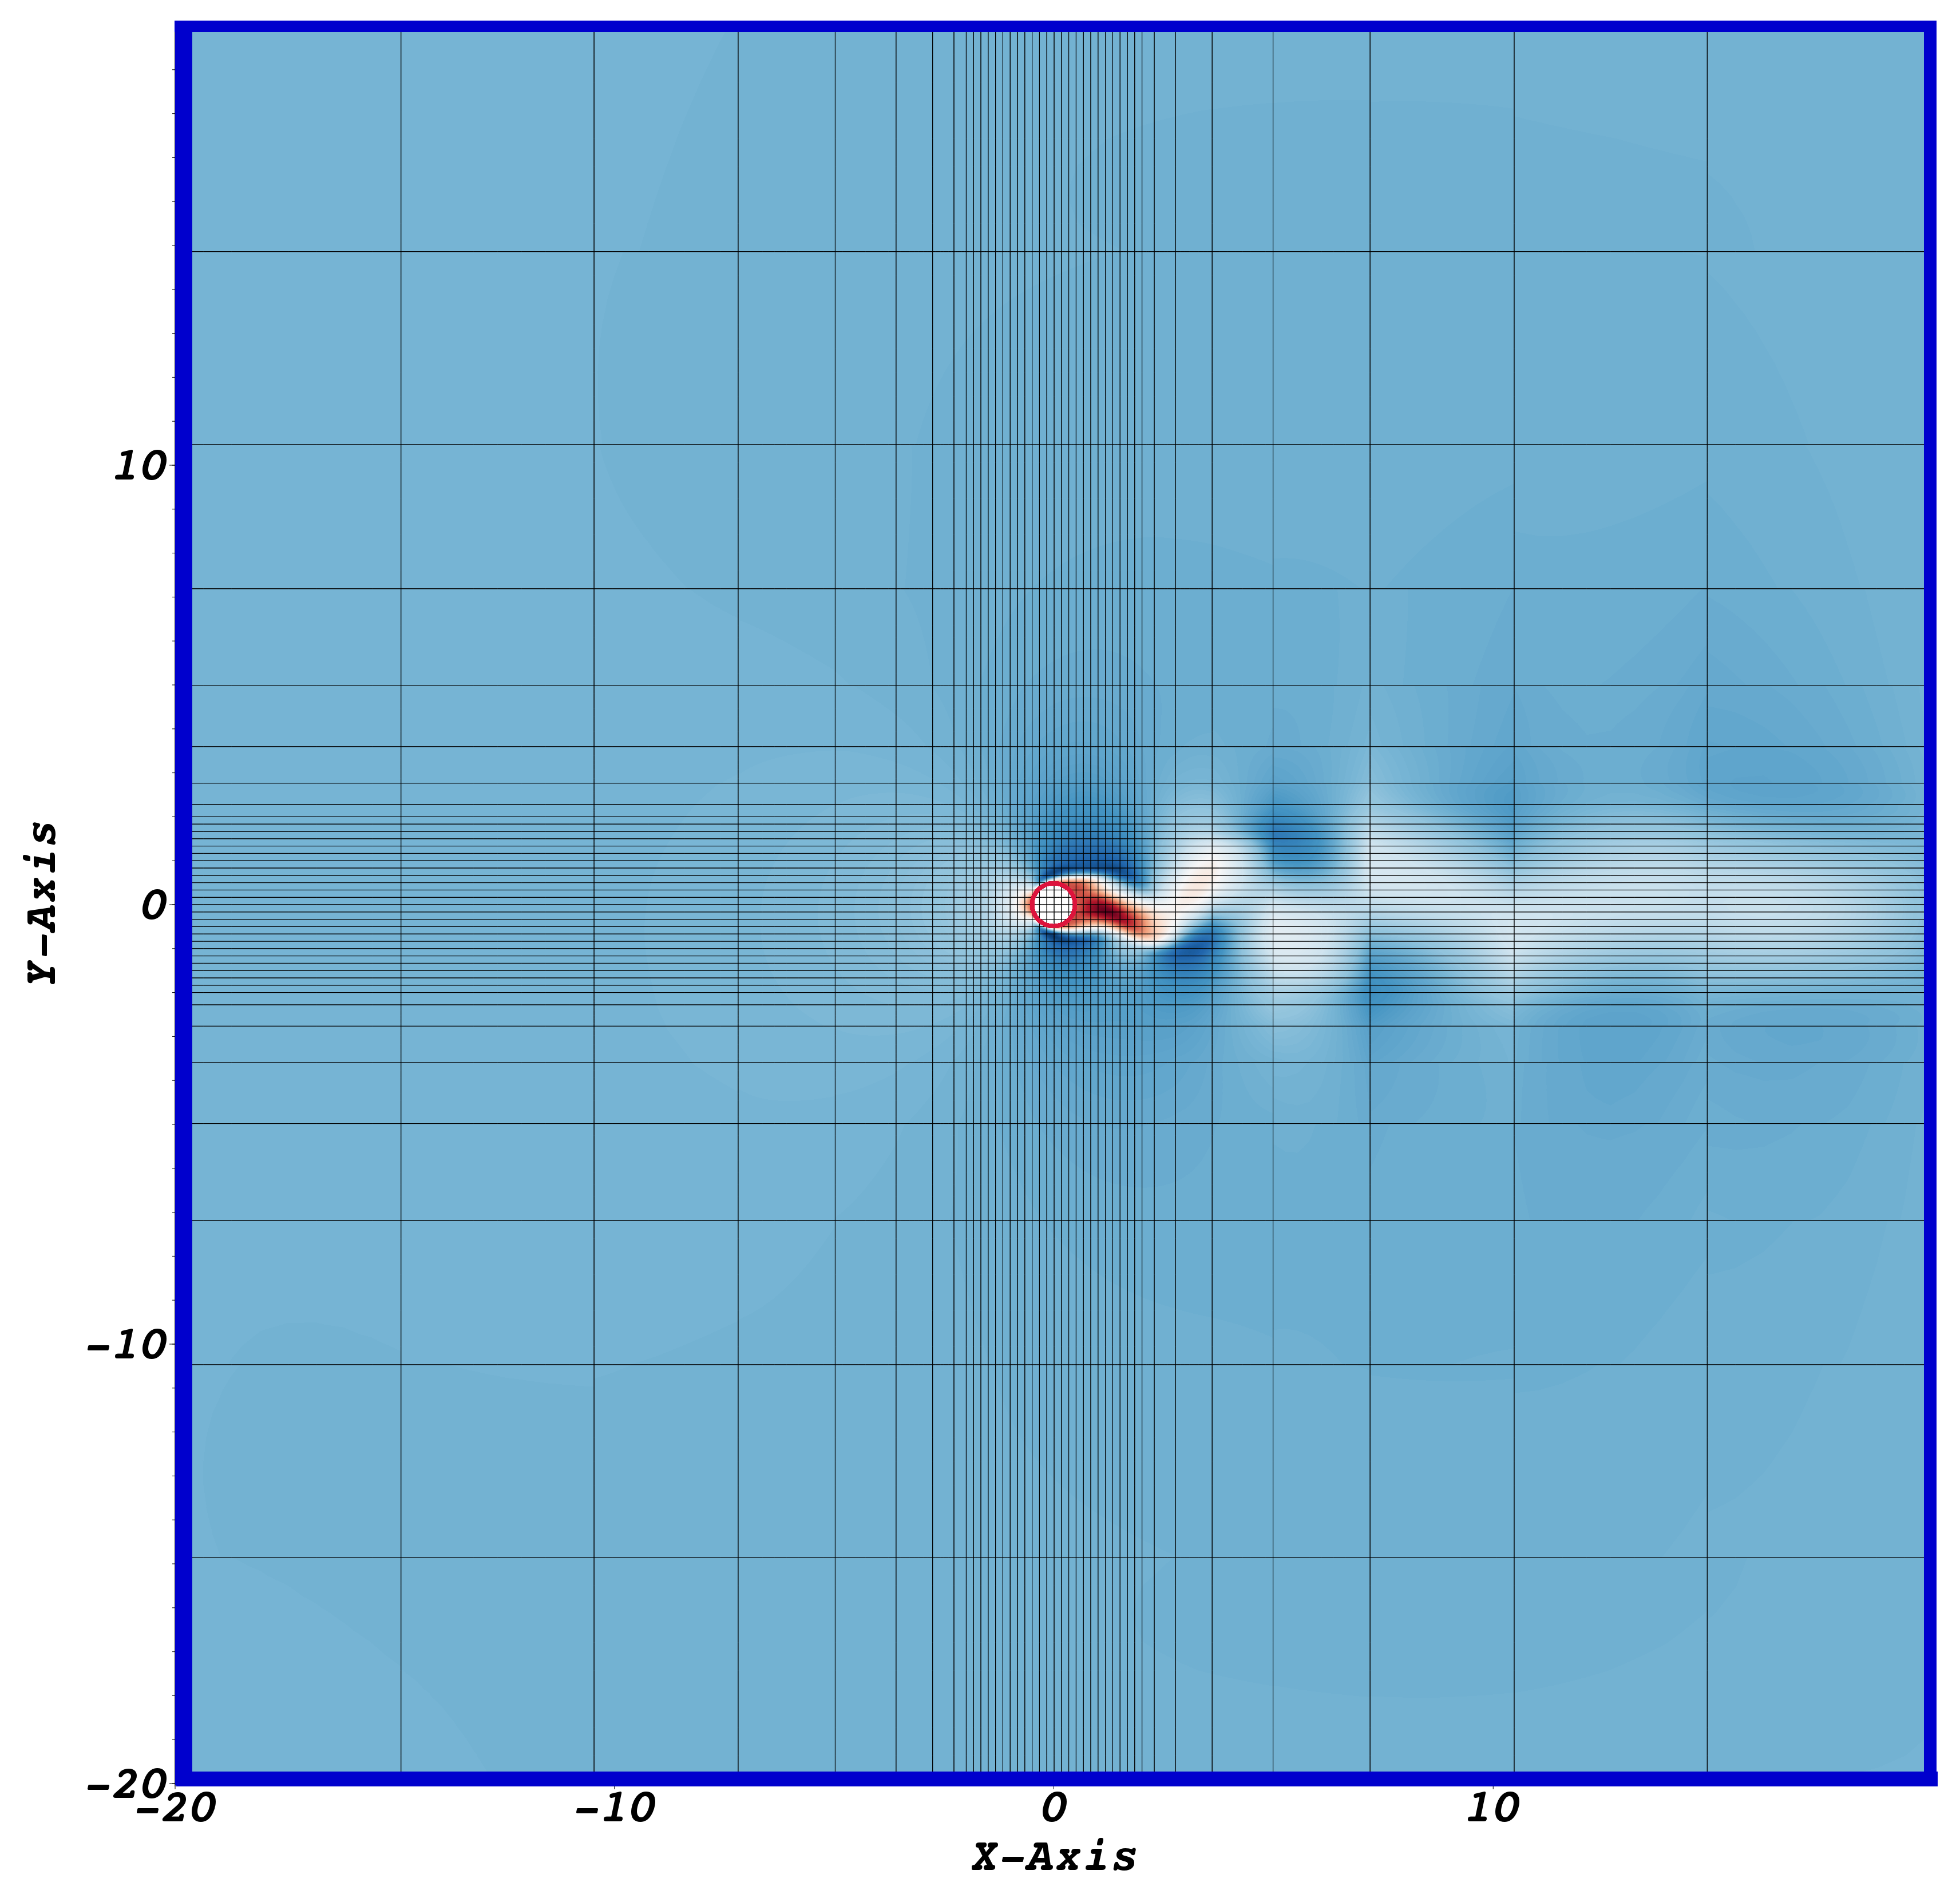
\includegraphics[width=\textwidth]{img/mesh40.PNG}
				\caption{Coarsest mesh with $40 \times 40$ cells}
			\end{figure} 
%			\begin{itemize}
%				\bluedot Supersonic inlet
%				\reddot Isothermal wall
%			\end{itemize}
		\end{columns}
%			simulation parameter
%			gitter
%			cD, CL, W*, St
		\end{frame}
		\begin{frame}
			\frametitle{Compared Values}
				\begin{columns}
					\column[]{8cm}
			
			\begin{itemize}			
				\item Steady flow simulations for $\text{Re = 20}$ and $\text{Re = 40}$:
				\begin{itemize}
					\item Coefficient of drag $C_D$
					\item Wake separation length $W^*$ \newline \MVRightArrow \, found from evaluating $x$ at $y=0$ where $x$-velocity $u=0$
				\end{itemize}
				\pause
				\item Unsteady flow simulations for $\text{Re = 100}$ and $\text{Re = 200}$:
				\begin{itemize}
					\item Coefficient of drag $C_D$
					\item Coefficient of lift $C_L$
					\item $\text{St}$ found from evaluating frequency of $C_L$
				\end{itemize}	
			\end{itemize}	
			\column[]{4cm}
			\onslide
			\begin{flalign*}
				C_D &= \tfrac{d}{q_\infty L_\infty}\\
				C_L &= \tfrac{l}{q_\infty L_\infty}\\
				\text{St} &= \dfrac{f L_\infty}{V_\infty}\\
				d&: 	\text{drag force}\\
				l&:	\text{lift force}\\
				q_\infty&:	\text{dynamic pressure}\\
				L_\infty&: \text{cylinder diameter}\\
				V_\infty&: \text{flow velocity}\\
			\end{flalign*}
			\end{columns}
		\end{frame}
		\begin{frame}[allowframebreaks]
			\frametitle{Simulation at $\text{Re = 20}$}
			\begin{table}[htp]
				\small
				\centering
				\begin{tabular}{|l|l|c|c|c|}
					\hline
					\rule{0pt}{2,3ex}$\text{Re}=20$                              & Source                             & 2D/3D & $W^*$ & $C_D$ \\ \hline
					\rule{0pt}{2,3ex}\multirow{3}{*}{\begin{minipage}{2.8cm}Numerical --\newline Incompressible\end{minipage}} & Dennis and Chang           & 2D    & $0.94$     & $2.05$     \\ \cline{2-5} 
					\rule{0pt}{2,3ex}& Fornberg                 & 2D    & $0.91$     & $2.00$     \\ \cline{2-5} 
					\rule{0pt}{2,3ex}& Linnick and Fasel         & 2D    &$ 0.93 $    & $2.06$     \\ \hline
					\rule{0pt}{2,3ex}\multirow{2}{*}{Experimental}               & Coutanceau and Bouard       & -     & 0.93    & -     \\ \cline{2-5} 
					\rule{0pt}{2,3ex}& Tritton             & -     & -     & $2.09$     \\ \hline
					\rule{0pt}{2,3ex}\multirow{3}{*}{\begin{minipage}{2.8cm}Numerical --\newline Compressible\end{minipage}}     & Brehm, Hader and Fasel (Ma = 0.1) & 3D    & $0.96$     &$ 2.02$     \\ \cline{2-5} 
					\rule{0pt}{2,3ex}& Ayers                 & 2D    & $0.975$     & $2.06 $    \\ \cline{2-5} 
					\rule{0pt}{2,3ex}& \textbf{Present Results:}                   & \textbf{2D}    & $\mathbf{0.928}$     & $\mathbf{2.136}$     \\ \hline
				\end{tabular}	
			\end{table}
			\begin{itemize}
				\item $W^*$ coincides with literature, $C_D$ much too high
			\end{itemize}
		%	re 20 tabelle, plot, drag over time, vorticity
%		\end{frame}
%		\begin{frame}
\vspace{4cm}
			\begin{columns}[t]
				\column[]{5cm}
				\begin{itemize}
					\item None of the values lies in the range found in literature
					\item Simulation for $P=2$, $\text{CpD}=80$ should be examined again
					\item Overall, $P=1$ behaviour as expected,  $P=2$ and $3$ yield much too high results
				\end{itemize}
				\column[]{7cm}
				\begin{figure}[htp]
					\centering		
					\includestandalone[width=\textwidth]{re20cdwerte}
				\end{figure}
			\end{columns}
		\end{frame}
		\begin{frame}[allowframebreaks]
			\frametitle{Simulation at $\text{Re = 40}$}
			\begin{table}[htp]
				\small
				\centering
				\begin{tabular}{|l|l|c|c|c|}
					\hline
					\rule{0pt}{2,3ex}$\text{Re}=40$                              & Source                             & 2D/3D & $W^*$ & $C_D$ \\ \hline
					\rule{0pt}{2,3ex}\multirow{3}{*}{\begin{minipage}{2.8cm}Numerical --\newline Incompressible\end{minipage}} & Dennis and Chang          & 2D    & $2.35$     & $1.52 $    \\ \cline{2-5} 
					\rule{0pt}{2,3ex}& Fornberg                & 2D    & $2.24$     & $1.50 $   \\ \cline{2-5} 
					\rule{0pt}{2,3ex}& Linnick and Fasel         & 2D    &$ 2.28$     & $1.54  $   \\ \hline
					\rule{0pt}{2,3ex}\multirow{2}{*}{Experimental}               & Coutanceau and Bouard      & -     & $2.13 $  & -     \\ \cline{2-5} 
					\rule{0pt}{2,3ex}& Tritton                & -     & -     & $1.59 $    \\ \hline
					\rule{0pt}{2,3ex}\multirow{3}{*}{\begin{minipage}{2.8cm}Numerical --\newline Compressible\end{minipage}}     & Brehm, Hader and Fasel (Ma = 0.1) & 3D    & $2.26$     & $1.51 $    \\ \cline{2-5} 
					\rule{0pt}{2,3ex}& Ayers                 & 2D    & $2.250 $    & $1.605$     \\ \cline{2-5} 
					\rule{0pt}{2,3ex}& \textbf{Present Results:}                   & \textbf{2D}    & $\mathbf{2.201}$     & $\mathbf{1.608} $    \\ \hline
				\end{tabular}	
			\end{table}
			\begin{itemize}
				\item $W^*$ coincides with literature, $C_D$ slightly high
			\end{itemize}
%			re 40 tabelle, plot, drag over time, vorticity 
%		\end{frame}
%		\begin{frame}
\vspace{1cm}
			\begin{columns}[t]
				\column[]{5cm}
				\begin{itemize}
					\item Better results than for $\text{Re=20}$
					\item Simulation for $P=2$, $\text{CpD}=80$ once again yields discordant values
					\item $P=2$ and $P=3$ quite high compared to literature
				\end{itemize}
				\column[]{7cm}
				\begin{figure}[htp]
					\centering		
					\includestandalone[width=\textwidth]{re40cdwerte}
				\end{figure}
			\end{columns}
		\end{frame}
		\begin{frame}
			\frametitle{Comparison of $\text{Re = 20}$ and $\text{Re = 40}$}
			\begin{center}
		\vspace{-0.3cm}
			\scalebox{0.8}{
				\begin{minipage}{\the\textwidth}
			\begin{table}[htp]
				\begin{tabular}{|c|c|c|}
					\hline
					& $W^*$   & $C_D$   \\ \hline
					$\text{Re}=20$ & $0.928$ & $2.136$ \\ \hline
					$\text{Re}=40$ & $2.201$ & $1.608$ \\ \hline
				\end{tabular}
			\end{table}
		\end{minipage}
		}
	\end{center}
			\begin{figure}
				\vspace{-0.5cm}
				\centering
				\subfloat[$\text{Re = 20}$]{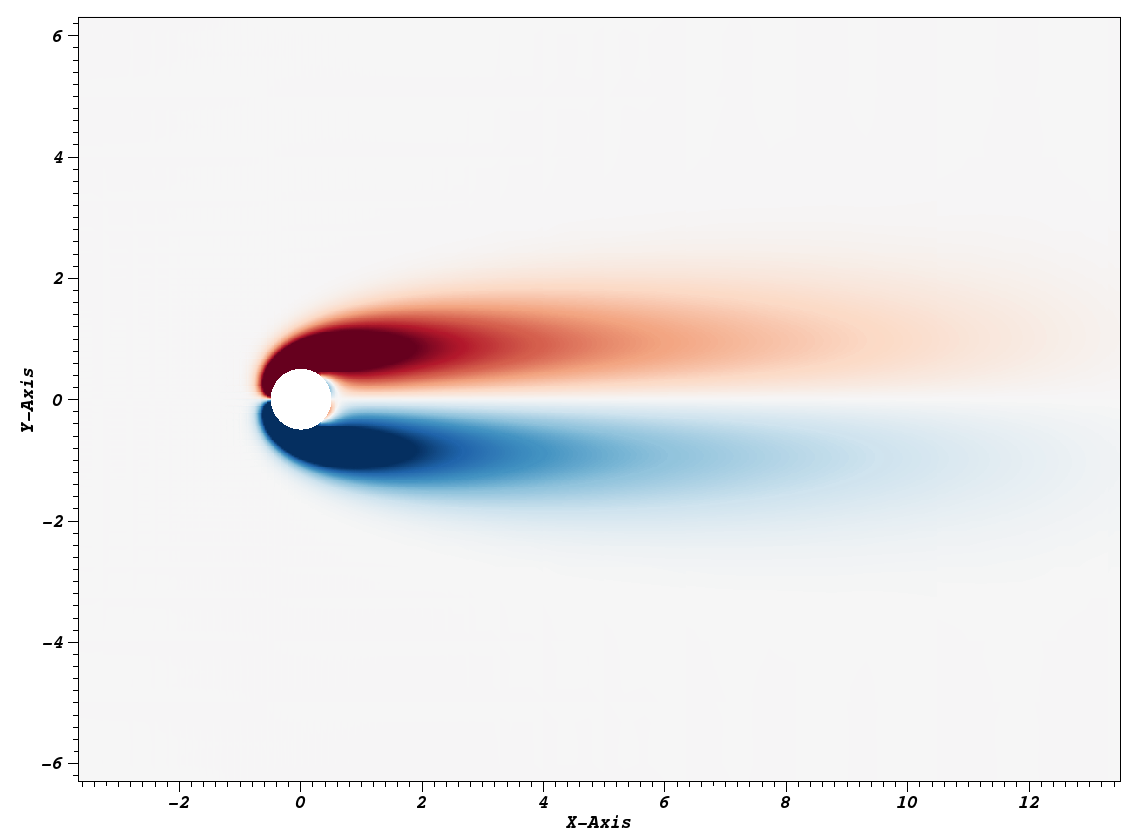
\includegraphics[width=0.45\textwidth]{img/Re20DG3CpD60.png}}
				\subfloat[$\text{Re = 40}$]{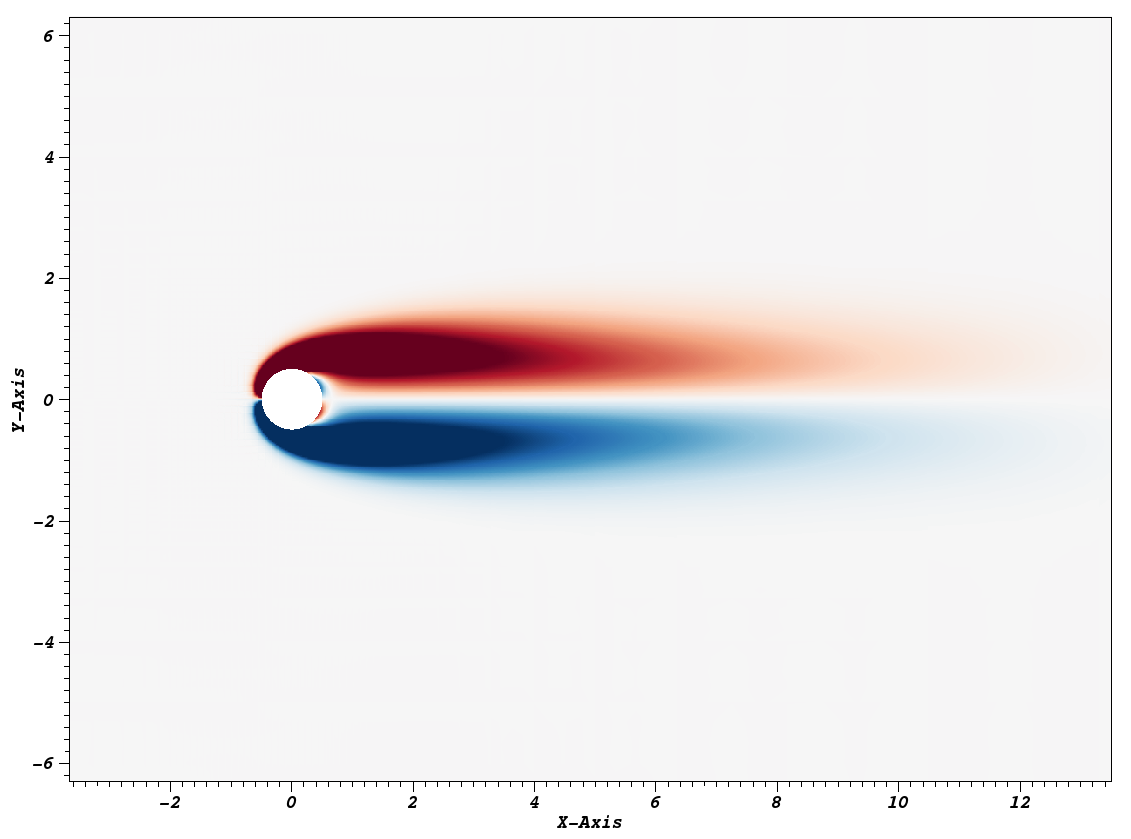
\includegraphics[width=0.45\textwidth]{img/Re40DG3CpD60.png}}
			\end{figure}
	\end{frame}
		\begin{frame}[allowframebreaks]
			\frametitle{Simulation at $\text{Re = 100}$}
			\vspace{-0.3cm}
			\scalebox{0.7}{
					\begin{minipage}{\the\textwidth}
			\begin{table}[htp]
				\centering
				\begin{tabular}{|l|l|c|c|c|c|}
					\hline
					\rule{0pt}{2,3ex}$\text{Re}=100$                              & Source                             & 2D/3D & $St$ & $C_D$ & $C_L$\\ \hline
					\rule{0pt}{2,3ex}\multirow{7}{*}{\begin{minipage}{2.8cm}Numerical --\newline Incompressible\end{minipage}} & Gresho, Chan, Lee, et al.           & 2D    & $0.18$     & $1.76$ & -   \\ \cline{2-6} 
					\rule{0pt}{2,3ex}& Linnick and Fasel ($\lambda = 0.056$)                 & 2D    & $0.169$     & $1.38 \pm 0.010$  &  $\pm  0.337 $\\ \cline{2-6} 
					\rule{0pt}{2,3ex}& Linnick ad Fasel ($\lambda = 0.023$)                  & 2D    & $0.1696 $   & $1.34 \pm 0.009$  & $ \pm 0.333 $\\ \cline{2-6} 
					\rule{0pt}{2,3ex}& Persillon and Braza                  & 2D    & $0.165  $   &$ 1.253 $ & -  \\ \cline{2-6} 
					\rule{0pt}{2,3ex}& Saiki and Biringen                 & 2D    &$ 0.171  $   & $1.26 $ &  - \\ \cline{2-6} 
					\rule{0pt}{2,3ex}& Persillon and Braza                   & 3D    & $0.164$     & $1.240 $ & -  \\ \cline{2-6} 
					\rule{0pt}{2,3ex}& Liu, Zheng and Sung         & 3D    &$ 0.165 $    & $1.35 \pm 0.012$  &$ \pm 0.339 $ \\ \hline
					\rule{0pt}{2,3ex}\multirow{2}{*}{Experimental}               & Berger and Wille     & -     &$ 0.16-0.17 $   & -    & -\\ \cline{2-6} 
					\rule{0pt}{2,3ex}& Clift, Grace and Weber               & -    & -     &$ 1.24 $ &  - \\ \cline{2-6} 
					\rule{0pt}{2,3ex}& Williamson              & -     &$ 0.164  $  & -   & - \\ \hline
					\rule{0pt}{2,3ex}\multirow{3}{*}{\begin{minipage}{2.8cm}Numerical -- \newline Compressible\end{minipage}}     & Brehm, Hader and Fasel (Ma = 0.1) & 3D    & $0.165$    &$ 1.32 \pm 0.01  $  & $\pm 0.32 $\\ \cline{2-6} 
					\rule{0pt}{2,3ex}& Ayers                  & 2D    &$ 0.167$     & $1.371 \pm 0.011 $ &$ \pm 0.333 $\\ \cline{2-6} 
					\rule{0pt}{2,3ex}& \textbf{Present Results:}                   & \textbf{2D}    & $\mathbf{0.1669}$     & $\mathbf{1.3593 \pm 0.00805}$  &  $\mathbf{\pm 0.3291}$ \\ \hline
				\end{tabular}	
			\end{table}
				\end{minipage}
			}
			\vspace{-0.1cm}
			\begin{itemize}
				\item All values coincide with literature
			\end{itemize}
%			
			\begin{columns}[t]
				\column[]{5cm}
				\begin{itemize}
					\item Higher degree values lie in expected range
					\item Values which should be most accurate ($P=2$, $\text{CpD}=80$ and $P=3$, $\text{CpD}=60$) produce rather high results
					\item $P=2$ seems to converge against $P=3$, $\text{CpD}=60$ value
				\end{itemize}
				\column[]{7cm}
				\begin{figure}[htp]
					\centering		
					\includestandalone[width=\textwidth]{re100cdwerte}
				\end{figure}
			\end{columns}
			
		\end{frame}
		\begin{frame}[allowframebreaks]
			\frametitle{Simulation at $\text{Re = 200}$}
			\scalebox{0.7}{
				\begin{minipage}{\the\textwidth}
			\begin{table}[htp]
				\centering
				\begin{tabular}{|l|l|c|c|c|c|}
					\hline
					\rule{0pt}{2,3ex}$\text{Re}=200$                              & Source                             & 2D/3D & $St$ & $C_D$ & $C_L$\\ \hline
					\rule{0pt}{2,3ex}\multirow{9}{*}{\begin{minipage}{2.8cm}Numerical --\newline Incompressible\end{minipage}} & Belov, Martinelli and Jameson           & 2D    & $0.193$     & $1.19 \pm 0.042$ & $\pm 0.64$   \\ \cline{2-6} 
					\rule{0pt}{2,3ex} & Gresho, Chan, Lee et al.             & 2D    & $0.21$     & $1.76$ & -   \\ \cline{2-6} 
					\rule{0pt}{2,3ex}& Linnick and Fasel ($\lambda = 0.056$)                 & 2D    & $0.199$     & $1.37 \pm 0.046$  &  $\pm  0.70$\\ \cline{2-6} 
					\rule{0pt}{2,3ex}& Linnick and Fasel ($\lambda = 0.023$)                  & 2D    & $0.197 $   & $1.34 \pm 0.044$  & $ \pm 0.69$\\ \cline{2-6} 
					\rule{0pt}{2,3ex}& Miyake, Sakamoto, Tokunaga et al.               & 2D    & $0.196$   &$1.34 \pm 0.043 $ & $\pm 0.67$  \\ \cline{2-6} 
					\rule{0pt}{2,3ex}&  Persillon and Braza               & 2D    & $0.198  $   &$ 1.321 $ & -  \\ \cline{2-6} 
					\rule{0pt}{2,3ex}& Saiki and Biringen                 & 2D    &$ 0.197  $   & $1.18 $ &  - \\ \cline{2-6} 
					\rule{0pt}{2,3ex}& Persillon and Braza                 & 3D    & $0.181$     & $1.306 $ & -  \\ \cline{2-6} 
					\rule{0pt}{2,3ex}& Liu, Zheng and Sung           & 3D    &$ 0.192 $    & $1.31 \pm 0.049$  &$ \pm 0.69 $ \\ \hline
					\rule{0pt}{2,3ex}\multirow{2}{*}{Experimental}               & Berger and Wille      & -     &$ 0.18-0.19 $   & -    & -\\ \cline{2-6} 
					\rule{0pt}{2,3ex}& Clift, Grace and Weber                 & -    & -     &$ 1.16 $ &  - \\ \cline{2-6} 
					\rule{0pt}{2,3ex}& Williamson               & -     &$ 0.181  $  & -   & - \\ \hline
					\rule{0pt}{2,3ex}\multirow{3}{*}{\begin{minipage}{2.8cm}Numerical --\newline Compressible\end{minipage} }    &  Brehm, Hader and Fasel (Ma = 0.1) & 3D    & $0.192$    &$ 1.3 \pm 0.04  $  & $\pm 0.66 $\\ \cline{2-6} 
					\rule{0pt}{2,3ex}& Ayers                  & 2D    &$ 0.201$     & $1.371 \pm 0.011 $ &$ \pm 0.70 $\\ \cline{2-6} 
					\rule{0pt}{2,3ex}& \textbf{Present Results:}                   & \textbf{2D}    & $\mathbf{0.2002}$     & $\mathbf{1.344 \pm 0.0462}$  &   $\mathbf{\pm 0.6887}$\\ \hline
				\end{tabular}	
			\end{table}
		\end{minipage}
		}
			\begin{columns}[t]
				\column[]{5cm}
				\begin{itemize}
					\item All values seen in table coincide with literature
					\item Compared to 3D results by \cite[Brehm et al.]{brehm} all values slightly higher
					\item All $C_D$ values (except for the least accurate one) lie in expected range
					\item $P=2$ seems to converge against higher value than $P=1$
				\end{itemize}
				\column[]{7cm}
				\begin{figure}[htp]
					\centering		
					\includestandalone[width=\textwidth]{re200cdwerte}
				\end{figure}
			\end{columns}
		\end{frame}
		\begin{frame}[allowframebreaks]
			\frametitle{Comparison of $\text{Re = 100}$ and $\text{Re = 200}$}
			\begin{columns}[t]
				\column[]{6.5cm}
				\vspace{-1cm}
				\begin{figure}[htp]
					\centering		
					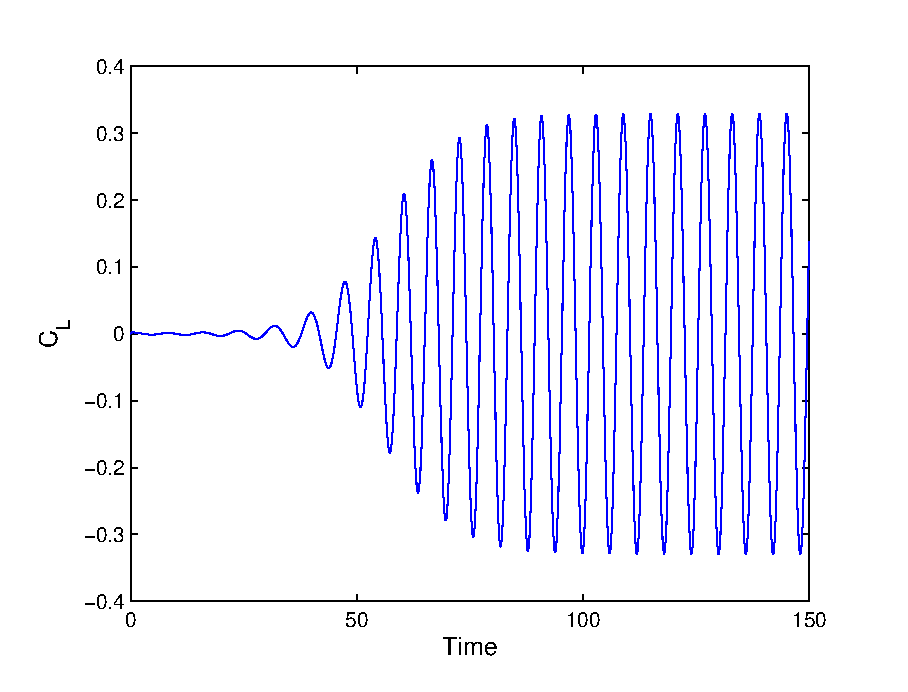
\includegraphics[width=\textwidth]{img/re100dg3cpd60cl.eps}
				\end{figure}
%				\vspace{-0.5cm}

				\column[]{6.5cm}
				\vspace{-1cm}
			\begin{figure}[htp]
				\centering		
				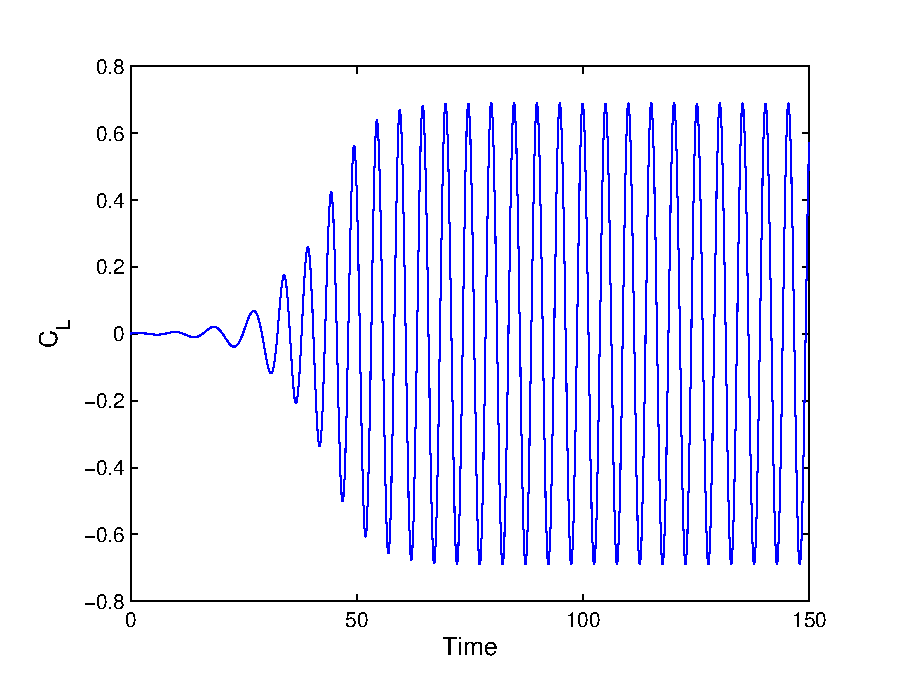
\includegraphics[width=\textwidth]{img/re200dg3cpd60cl.eps}
			\end{figure}
			\end{columns}
			\begin{itemize}
				\item Higher amplitude and frequency for $C_L$ at $\text{Re}=200$ compared to $\text{Re}=100$
				\item Steady state is reached earlier
			\end{itemize}
			\vspace{5cm}
			\begin{columns}[t]
				\column[]{6cm}
				\vspace{-1cm}
				\begin{figure}[htp]
					\centering		
					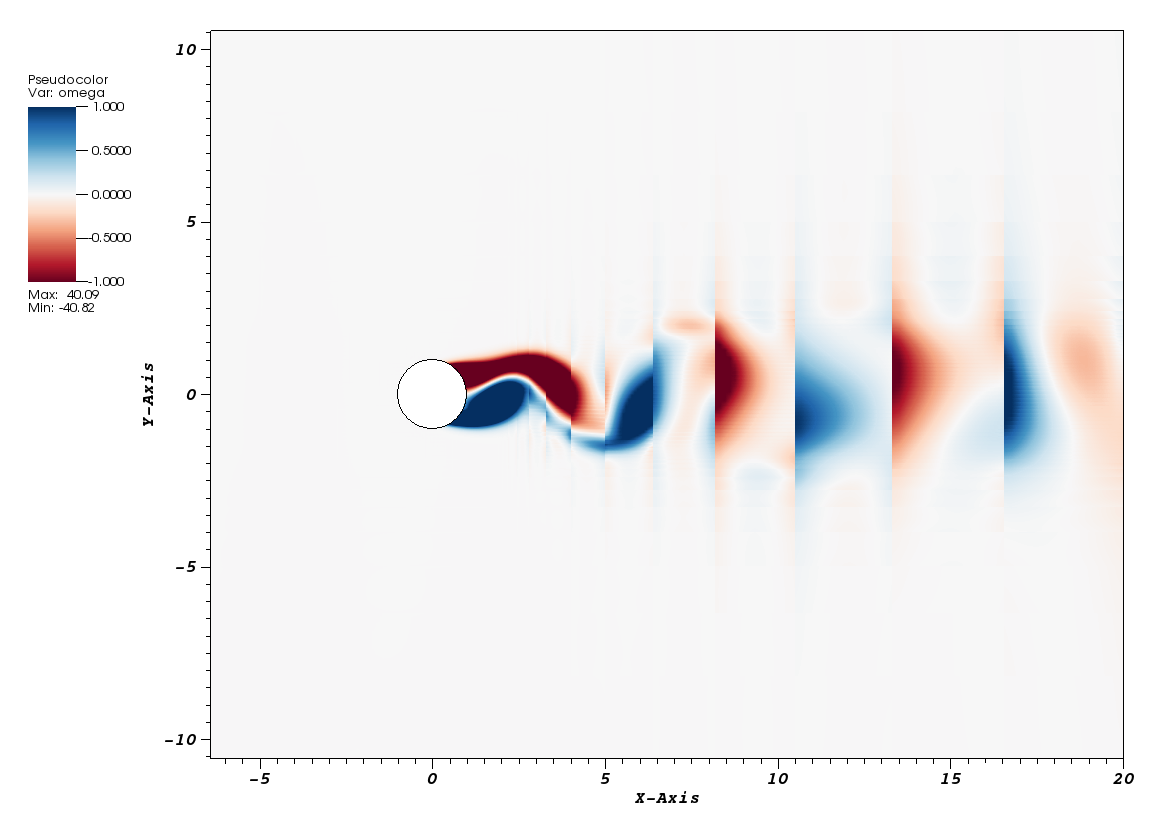
\includegraphics[width=\textwidth]{img/re100dg3cpd60.png}
				\end{figure}
				\column[]{6cm}
				\vspace{-1cm}
				\begin{figure}[htp]
					\centering		
					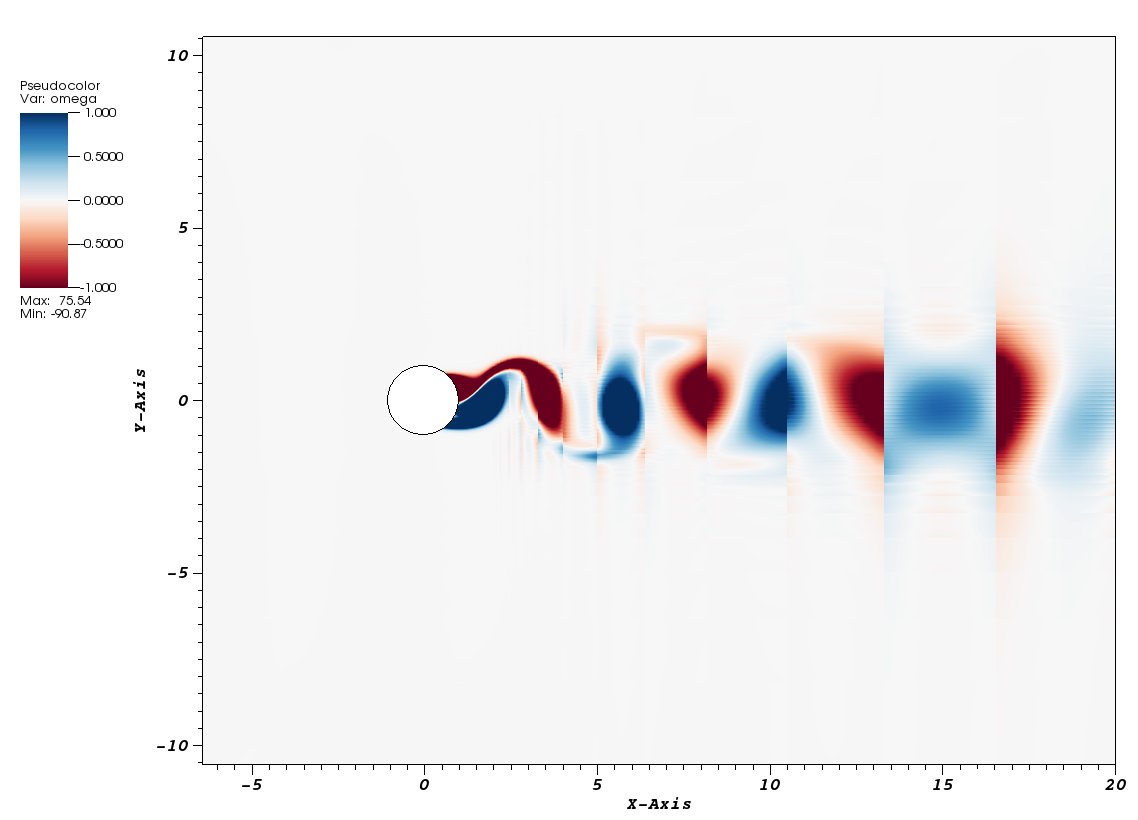
\includegraphics[width=\textwidth]{img/re200dg3cpd60.png}
				\end{figure}
			\end{columns}
			\begin{center}
			\scalebox{0.8}{
				\begin{minipage}{\the\textwidth}
					\begin{table}[htp]
						\begin{tabular}{|c|c|c|c|}
							\hline
							& $St$   & $C_D$  & $C_L$ \\ \hline
							$\text{Re}=100$ & $0.1669$ & $1.359\pm 0.00805$ & $\pm 0.3291$ \\ \hline
							$\text{Re}=200$ & $0.2002$ & $1.344 \pm 0.0462$ & $\pm 0.6887$ \\ \hline
						\end{tabular}
					\end{table}
				\end{minipage}
			}
		\end{center}
		\end{frame}
\section{Conclusion and Outlook}
\frame{\tableofcontents[currentsection]}
		\begin{frame}
			\frametitle{Summary}
			conclusion
		\end{frame}
		\begin{frame}
			\frametitle{Outlook}
			future works
		\end{frame}
		
		\begin{frame}
			\frametitle{The End}
			ende, fragen
		\end{frame}
		\begin{frame}
			\frametitle{Bibliography}
			bibliography
		\end{frame}		
	
\appendix
%\newcounter{finalframe}
%\setcounter{finalframe}{\value{framenumber}}
%% Backup frames
%\setcounter{framenumber}{\value{finalframe}}
		\begin{frame}
			alle tabellen und graphen die man brauchen könnte in anhang
		\end{frame}		
\begin{frame}

\end{frame}
\end{document}

